\section{Implementation}
\label{implementation}

This chapter describes the implementation part of the thesis. A literature review was conducted to research best practices for compiling C/C++ to JavaScript and WebAssembly.
% \hl{modules(are modules described?)}. 
The result of the implementation is a technical artifact in the form of a benchmarking suite (prototype). The progression chapter provides guidelines for any individual that wishes to repeat the development of the technical artifact. The source code of the the artifact is available on Github\footnote{\url{https://github.com/a17danos/implementation/}}. The end of the chapter describes a small pilot study where the benchmarking suite was used to gather data that was processed using a spreadsheet application to conclude if WebAssembly provides a significant performance improvement over JavaScript for the provided use cases.

\subsection{Literature review}

This thesis focuses on WebAssembly, JavaScript, asm.js, and benchmarking performance. Academic literature on WebAssembly is sparse. Primary sources such as scientific articles, conference papers was researched in multiple databases such as ACM Digital Library, IEEE Xplore and Scopus using combinations of the keywords \texttt{webassembly}, \texttt{wasm}, \texttt{javascript}, \texttt{asm.js}, \texttt{benchmarking}, and \texttt{performance}. ACM Digital Library and IEEE Xplore returned the most articles. Articles was evaluated based on the author, skimming the abstract, and by the manually evaluating the reliability of the journal or conference the articled was published in. Most articles has been referenced throughout this thesis including the principal paper from \textcite{HaasRossbergSchuffTitzerHolmanGohmanWagnerZakaiBastien2017}. There are no \emph{primary} sources that describe best practices for working with WebAssembly. This is a reasonable, but not ideal, situation which is due to the fact that WebAssembly was made public less than two years ago. Secondary sources was researched by searching for the same keywords and in combination with the keyword \texttt{book} in Google search. Only a handful of books was found: \textcite{Barker2012,Rourke2018,Gallant2019} of which the last one is currently only available as part of a early access program. There is a vast amount of ternary sources on WebAssembly available in the form of documentation, articles published on personal blogs and Medium, Github issues, and YouTube videos just to mention a few. The next two sections describes the technical artifact and it's progression referencing secondary sources in combination with references to commits of the technical artifact pushed to the central repository on Github in the form of footnotes.

%can I use hashes in parentheses instead of footnotes when referring to Github?

\subsection{Technical artifact}

%\hl{/EMCAScript vX}. \hl{The benchmarking suite has been named membrane, below variants of (technical) artifact, (benchmarking) suite, and membrane is used to describe ''it''.}

The technical artifact is implemented as a simple benchmarking suite using HTML, CSS and JavaScript implemented in a single file called \texttt{membrane.html}. The benchmarking suite measures the time it takes to execute use cases compiled as wasm from \texttt{membrane.wasm} and compiled as asm.js from \texttt{membrane.asm.js}. Time is measured using performance.now(), as in perfLogger \parencite{Barker2012}. 

%Figure \ref{membrane} shows a screenshot of the benchmarking suite on the April 22, 2019\footnote{\url{https://github.com/a17danos/implementation/tree/98cee52}}. 

The design is designed to be elementary with only necessary elements. The intention is that the straightforward design puts the focus on the content. Content consist of three labels and two tables. The top table shows descriptive statistics and the bottom table contains all data gathered from measuring performance. The descriptive statistics shown are best (lowest) time, the worst (highest) time, the average (arithmetic mean) time, and the standard deviation (for the sample). The use of html table elements provides good support for copy and pasting data from a web page into a spreadsheet. Initially a function to let the user download a file of comma separated values (csv) was planned, but this plan was dropped due to potential errors handling such files in different web browsers, operating systems and spreadsheet software. The implementation of membrane.html is trivial with exception of initializing and executing code\footnote{\url{https://github.com/a17danos/implementation/commit/98cee52}} from referenced wasm and asm.js files as seen Listing \ref{membrane-core.html}.

\lstinputlisting[label=membrane-core.html,language=html,caption=membrane-core.html]{../Listings/membrane-core.html}

%https://github.com/Apress/pro-javascript-perf/blob/master/source%20code/perfLogger/perfLogger.js

\begin{comment}
\begin{figure}[!h]
\centering
%\fbox{
\includegraphics[width=16cm,keepaspectratio]{../Figures/membrane}
%}
\caption{The technical artifact in the form of a benchmarking suite named membrane.}
\label{membrane}
\end{figure}
\end{comment}

% TODO: describe internals of membrane.html including measuring time using Performance.mark()

The wasm file \texttt{membrane.wasm} and the asm.js file \texttt{membrane.asm.js} are the result of a compilation, using Emscripten, of \texttt{membrane.cpp} that contains the use cases implemented as C/C++ source code. Figure \ref{membrane-implementation} illustrates the logical view of the implementation of the benchmarking suite. The two compiled files and implementation of membrane.html constitute the benchmarking suite while it can be argued that the technical artifact differs in that it includes the use case source code.

%(both commited to github along with instructions on how they were created).
 
\begin{figure}[!h]
\centering
%\fbox{
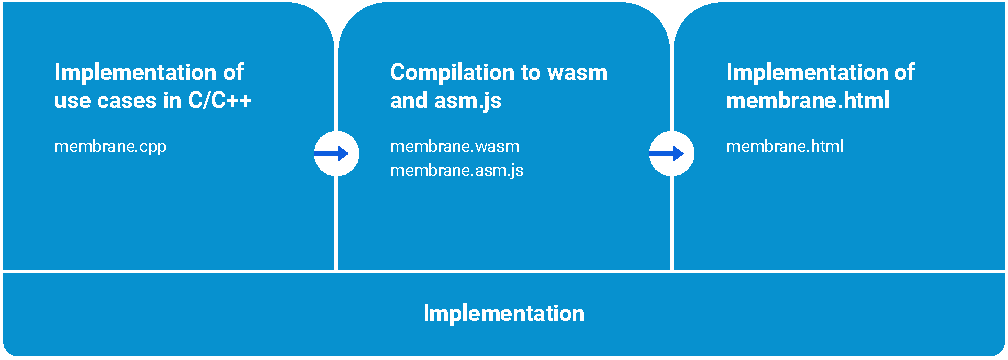
\includegraphics[width=16cm,keepaspectratio]{../Figures/membrane-implementation}
%}
\caption{The logical view of the implementation of the benchmarking suite.}
\label{membrane-implementation}
\end{figure}
    
The source code\footnote{\url{https://github.com/a17danos/implementation/}} for the technical artifact is available at Github and the membrane benchmarking suite\footnote{\url{https://a17danos.github.io/implementation/membrane.html}} is hosted using Github Pages\footnote{\url{https://pages.github.com/}}. Between April 2019 and April 2020 the domain membrane.site redirects to membrane.html on Github pages for easy entry in the location bar in web browsers, which is useful especially on mobile devices.

%The full source code for final version\footnote{\url{https://github.com/a17danos/implementation/tree/98cee52}} of the technical artifact is also included as a Appendix A. (ref to appendex that contains the screenshot and describes the git hash of the source code).

Much effort was put into researching the WebAssembly domain and testing and different tools. This effort is described more in detail in the next section.

% TODO: Add membrane.cpp listing

\subsection{Progression}

\begin{comment}
I progressions-kapitlet beskriver vi det en person som återupprepar arbetet behöver veta. Vilka viktiga designbeslut som tagits under processen samt hur dessa beslut implementerats. Eftersom programkoden och rapporten kommer ligga kvar under väldigt lång tid så innebär det att vi måste göra det så lätt som möjligt att följa hur arbetet utvecklats under genomförandet/implementationen. (Ett begränsat exempel på hur man kan lägga upp detta finns tillgängligt nedan).
\end{comment}

This section describes, on a high level, issues that was faced during the development of the technical artifact. Most of the issues could have been avoided with more understanding for the different tools and options available. This section aims to provide that understanding in general and discuss a few things in more detail.

The development of membrane started with exploring Emscripten SDK\footnote{\url{https://emscripten.org/docs/getting_started/downloads.html}}, the toolchain described at the developer guide at webassembly.org\footnote{\url{https://webassembly.org/getting-started/developers-guide/}}. Once Emscripten is installed C/C++ can be compiled to WebAssembly using \texttt{emcc}, e.g. \texttt{emcc hello.c -o hello.html}. Sometimes \texttt{em++} is referred to instead of \texttt{emcc}, the difference is that the former assumes C++ code while the latter looks at the file extension of the provided filename to determine if the code is C or C++. Emscripten was originally a tool to compile C/C++ to asm.js. Previous to version 1.38.1\footnote{\url{https://github.com/emscripten-core/emscripten/blob/incoming/ChangeLog.md\#v1381-05172018}} of Emscripten compiling to WebAssembly required the flag \texttt{WASM=1} to not output asm.js. The flag \texttt{WASM=1} is still common in both ternary sources as well as official Emscripten documentation.

By default Emscripten does not only produce a WebAssembly file but also additional resources based on the given output file extension. These additional resources contain helper methods and JavaScript code to invoke and pass data to and from WebAssembly. E.g. \texttt{emcc hello.c -o hello.html} will produce both a HTML file \emph{and} a JavaScript file while \texttt{emcc hello.c -o hello.wasm} only provides a JavaScript file of helper method and which requires the developer to write their own code to initialize and pass data to and from the WebAssembly module \parencite{Rourke2018}. Emscripten can also still be used to compile C/C++ to asm.js, e.g. \texttt{emcc hello.c -Os -Wseparate-asm -s WASM=0 -o hello.asm.js}, but to my knowledge there is no good way to invoke emcc \emph{once} to produce both asm.js \emph{and} WebAssembly without \emph{also} generating additional resources. The option \texttt{-Os} optimizes for code size, which includes removing any additional code otherwise added by Emscripten to allow passing of data to and from the WebAssembly. Optimizing for code size also means that functions that has not been marked as exported are also removed. With Emscripten there are at least two ways to mark functions as exported. 

\lstinputlisting[label=add.cpp,language=c++,caption=add.cpp]{../Listings/add.cpp}

The C++ file in Listing \ref{add.cpp} contains a function \texttt{add} that adds two integers. The function is prefixed with \texttt{EMSCRIPTEN\_KEEPALIVE} which keeps it from being removed despite any optimization and also exports the function so that it becomes available to invoke. nnn Without \texttt{EMSCRIPTEN\_KEEPALIVE} in the source file and with the option \texttt{-Os} passed to \texttt{emcc} the function would not be included in the wasm file. If no optimization flag is passed to \texttt{emcc} \texttt{EMSCRIPTEN\_KEEPALIVE} could be removed and the function \emph{could} still be included in the wasm file \emph{if} the method is exported using 
the \texttt{EXPORTED\_FUNCTIONS} emcc flag, e.g. \texttt{add.cpp -o add.wasm -s  EXPORTED\_FUNCTIONS="['\_add']"}. It's also worth noting that the macro \texttt{WASM\_EXPORT} in Listing \ref{add.cpp} is always required for C++ files, but is \emph{not} required for C files.

%https://github.com/a17danos/implementation/commit/98cee52

Besides Emscripten Clang, the LLVM\footnote{\url{http://releases.llvm.org/download.html}} compiler, can be used to produce wasm files without Emscripten. Clang compilation from C/C++ (really any LLVM-supported language) requires that \texttt{wasm32} and \texttt{wasm64} are registered as targets. This is the default since LLVM 8.0.0\footnote{\url{http://releases.llvm.org/8.0.0/docs/ReleaseNotes.html\#changes-to-the-webassembly-target}}. Invoke \texttt{llc --version} to verify which targets are supported and compile using something like \texttt{clang hello.c -o hello.wasm --target=wasm32 -nostdlib -Xlinker --no-entry -Xlinker\\ --allow-undefined}. To my knowledge Clang cannot produce asm.js and is thus not an option to use in this thesis.

Given the fast phase of WebAssembly and associated toolchains it's not uncommon that information regarding WebAssembly is inaccurate or incompatible with the latest version of the tools in use, such as \texttt{WASM=1} no longer being needed and Clang being able to produce WebAssembly by default. This includes some of the official documentation. It's recommended to look at the official list of compiler options and the release notes for the tool that is being used, such as the compiler options\footnote{\url{https://emscripten.org/docs/tools_reference/emcc.html}} and the release notes\footnote{\url{https://emscripten.org/docs/introducing_emscripten/release_notes.html}} for Emscripten.

\begin{table}[!h]
\caption{\label{toolchains}WebAssembly toolchains with the version used during the writing of this thesis.}
\centering
\begin{tabular}{ll}
\hline
\textbf{Name} & \textbf{Version} \\ \hline
Emscripten & 1.38.27 \\
LLVM (Clang) & 8.0.0 \\
Binaryen & 80 \\
WebAssembly Binary Toolkit & 1.0.10 \\ \hline
\end{tabular}
\end{table}
    
Besides Emscripten and LLVM/Clang there are other useful toolchains such as the WebAssembly Binary Toolkit\footnote{\url{https://github.com/WebAssembly/wabt/releases}} (wabt) and Binaryen\footnote{\url{https://github.com/WebAssembly/binaryen/releases}} (Figure \ref{toolchains}). WebAssembly Binary Toolkit contains useful tools such as \texttt{wasm2wat} to transform WebAssembly binary format\footnote{\url{https://webassembly.github.io/spec/core/binary/index.html}} to WebAssembly text format\footnote{\url{https://webassembly.github.io/spec/core/text/index.html}} and \texttt{wat2wasm} to transform WebAssembly text format to WebAssembly binary format. The two formats are described in Chapter 2 in \textcite{Rourke2018}. If the code in Listing \ref{add.cpp} would be compiled to wasm: \texttt{emcc add.cpp -o add.wasm -Os} the wasm binary file can then be converted to a wat text file: \texttt{wasm2wat add.wasm > add.wat}. The result is shown in Listing \ref{add.wat}.

\lstinputlisting[label=add.wat,language=c,caption=add.wat]{../Listings/add.wat}

The text format provides a human readable format that can be used to see which functions that are available, what they do, be used to change the implementation without the original source, and even as way of programming WebAssembly directly.

% https://github.com/AssemblyScript/assemblyscript

Binaryen is closely linked to Emscripten and contains tools such as \texttt{asm2wasm} and \texttt{wasm2js}. It also contains \texttt{binaryen.js} which is a JavaScript library to compile WebAssembly from a web browser. The possibility to compile source code from e.g. C/C++ into WebAssembly in a web browser is used by a number of tools such as WasmFiddle\footnote{\url{https://wasdk.github.io/WasmFiddle/}}, WebAssembly Explorer\footnote{\url{https://mbebenita.github.io/WasmExplorer/}}, and WebAssembly Studio\footnote{\url{https://webassembly.studio/}} as described by \textcite{Rourke2018}. This approach has the benefit that no toolchain is required locally and is thus recommended as a starting point.

Since web browsers prevents loading external files such as WebAssembly files the suite has to be served by a web server. One way of solving this locally is to use Emrun a small web server that is part of the Emscripten SDK, e.g. \texttt{emrun --no\_browser --port 8000 .}. Depending on the web development environment there could also be plugins available that provides such features such as the Live Server\footnote{\url{https://github.com/ritwickdey/vscode-live-server}} extension for VS Code\footnote{\url{https://code.visualstudio.com/docs/editor/extension-gallery}}, but depending on the way the WebAssembly module is loaded these web servers may not function correctly due to things such as the MIME type not being registered\footnote{\url{https://github.com/mdn/webassembly-examples/issues/5}}.

Depending on the application it me be useful to be able to disable WebAssembly support. This is possible in at least Chrome(ium) and Firefox\footnote{\url{https://github.com/stevespringett/disable-webassembly}}. Chrome requires a restart as it has to be started with additional flags, i.e. \texttt{chrome --js-flags=--noexpose\_wasm}. Firefox does not have this requirement and is thus recommended for scenarios where WebAssembly has to be disabled. To disable WebAssembly in Firefox go to \texttt{about:config} in Firefox and set the value of \texttt{javascript.options.wasm} to \texttt{false}. The changes should take effect immediately.

% TODO: can I make and index of links instead of having many many footnotes?

\clearpage

\subsection{Pilot study}
\subfile{pilot}
